\documentclass[tikz,border=2pt]{standalone}
\usepackage{amsmath,amssymb}
\usepackage{pgfplots}
\pgfplotsset{compat=1.18}
\usetikzlibrary{arrows.meta}
\begin{document}
% Pollaczek-Khinchine: E[W]/E[S] = (1+C_s^2)/2 * rho/(1-rho) for C_s^2 = 0 (M/D/1), 1/2, 1 (M/M/1).
% Marked: rho = 3/4, C_s^2 = 1/2 gives 2.25 (Example 1: E[S]=2 h, E[W]=4.5 h).
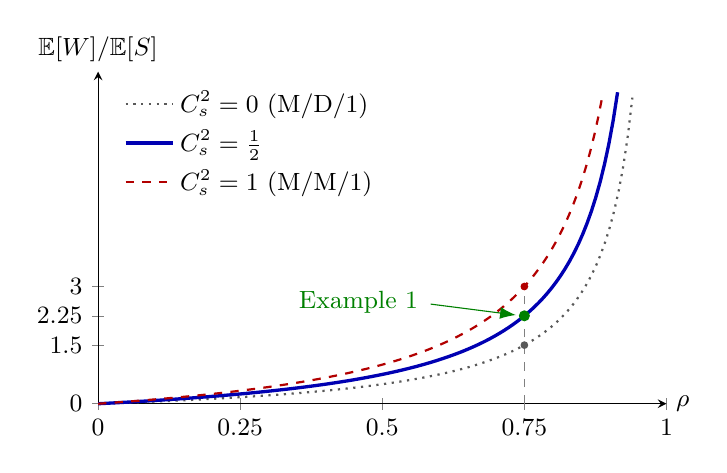
\begin{tikzpicture}[font=\small, >={Latex[length=2mm]}]
  \begin{axis}[
    axis lines=left, xmin=0, xmax=1.0, ymin=0, ymax=8.5,
    xtick={0,0.25,0.5,0.75,1}, xticklabels={$0$,$0.25$,$0.5$,$0.75$,$1$},
    ytick={0,1.5,2.25,3}, yticklabels={$0$,$1.5$,$2.25$,$3$},
    legend style={at={(axis cs:0.03,8.3)}, anchor=north west, draw=none, fill=none, row sep=1pt},
    legend cell align=left,
    xlabel={$\rho$}, ylabel={$\mathbb{E}[W]/\mathbb{E}[S]$},
    xlabel style={at={(axis description cs:1,0)}, anchor=west},
    ylabel style={rotate=-90, at={(axis description cs:0,1)}, anchor=south},
    samples=120, width=8.8cm, height=5.8cm, clip=false]
    \addplot[gray!70!black, thick, dotted, domain=0:0.94] {0.5*x/(1-x)};
    \addlegendentry{$C_s^2=0$ (M/D/1)}
    \addplot[blue!70!black, very thick, domain=0:0.914] {0.75*x/(1-x)};
    \addlegendentry{$C_s^2=\tfrac{1}{2}$}
    \addplot[red!70!black, thick, dashed, domain=0:0.888] {x/(1-x)};
    \addlegendentry{$C_s^2=1$ (M/M/1)}
    \draw[gray, thin, dashed] (axis cs:0.75,0) -- (axis cs:0.75,3);
    \fill[green!50!black] (axis cs:0.75,2.25) circle (2pt);
    \fill[gray!70!black] (axis cs:0.75,1.5) circle (1.4pt);
    \fill[red!70!black] (axis cs:0.75,3) circle (1.4pt);
    \node[green!50!black, anchor=east] at (axis cs:0.58,2.6) {Example 1};
    \draw[green!50!black, ->] (axis cs:0.585,2.55) -- (axis cs:0.735,2.27);
  \end{axis}
\end{tikzpicture}
\end{document}
